%%%%%%%%%%%%%%%%%%%%%%%%%%%%%%%%%%%%%%%%%%%
\subsection{Программное обеспечение для научных вычислений}
%%%%%%%%%%%%%%%%%%%%%%%%%%%%%%%%%%%%%%%%%%%
\begin{frame}
  \begin{figure}
    \centering
    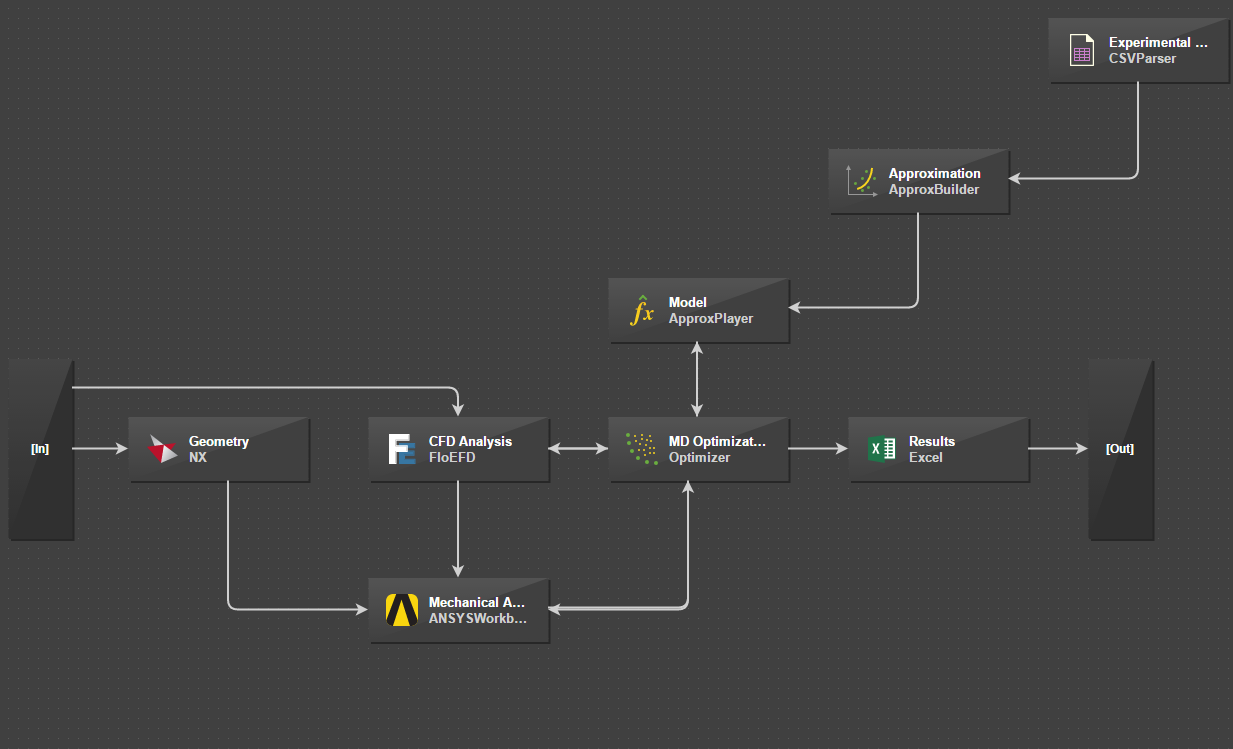
\includegraphics[width=\textwidth]{images/workflow1.png}
  \end{figure}

\end{frame}
%%%%%%%%%%%%%%%%%%%%%%%%%%%%%%%%%%%%%%%%%%%
\subsection{Научные системы организации рабочего процесса}
%%%%%%%%%%%%%%%%%%%%%%%%%%%%%%%%%%%%%%%%%%%
\begin{frame}



\end{frame}
%%%%%%%%%%%%%%%%%%%%%%%%%%%%%%%%%%%%%%%%%%%
\subsection{Современные подходы к организации вычислений}
%%%%%%%%%%%%%%%%%%%%%%%%%%%%%%%%%%%%%%%%%%%
\begin{frame}


\end{frame}
%%%%%%%%%%%%%%%%%%%%%%%%%%%%%%%%%%%%%%%%%%%
% --------------------------------------------------------------------------- %
\subsection{Цели и задачи разработки}
% --------------------------------------------------------------------------- %
\begin{frame}

  \begin{block}{Цель}
    Разработать программные средства для создания и интерпретации графовых описаний в программном каркасе comsdk.
  \end{block}

  \begin{block}{Задачи}
    \begin{enumerate}
      \item Провести сравнение объекта разработки с некоторым аналогичным.
      \item Сформировать требования к алгоритму, выполняющему этапы алгоритма по его описанию, составленному по методологии GBSE.
      \item Спроектировать структуры данных для описания и представления описаний алгоритмов и их элементов в программном каркасе comsdk.
      \item Разработать алгоритм обхода графовых моделей с использованием спроектированных структур данных.
      \item Представить интерфейсы или реализации разработанных алгоритмов и структур данных на языке С++.
    \end{enumerate}
  \end{block}

\end{frame}


